\chapter{Volume conductor theory}
\label{sec:VC}
\index{Volume conductor theory}
As we saw in the previous section, multicompartment (MC) models of morphologically complex neurons allow us to compute the transmembrane currents entering/leaving the neuron at various locations. This chapter is about how we, when we know the distribution of neuronal current sources, can use volume conductor (VC) theory to predict the extracellular potential at any given point in space. VC theory is the fundament for forward modeling of extracellular potentials at different spatial scales, from extracellular spikes, LFPs and MUAs, to ECoGs and EEGs.

Before we present the VC theory, we again want to emphasize that our scale of interest is a macroscopic one. When we talk about an extracellular current density or an extracellular potential, we will always refer to these quantities at a coarse-grained scale, i.e., as spatial averages over a volume of at least a cube micrometer. At this spatial scale we shall assume that the extracellular medium can be represented as a continuous medium \index{continuous medium} with an effective conductivity $\sigma_t$  \index{Conductivity}, representing the conductivity experienced by macroscopic extracellular currents through the tissue. Furthermore, we shall assume that an extracellular current density in this medium is linear and given by Ohm's law:
\begin{equation}
{\bf i_t}({\bf r}, t) = - \sigma_t({\bf r}, t) \nabla \phi({\bf r}, t),
\label{VC:eq:ohmici}
\end{equation}

Further discussion of the assumptions underlying VC theory are found at the end of this chapter (Section \ref{sec:VC:approximations}), and in Chapter \ref{sec:Sigma}, where we discuss the continuous medium approximation in greater detail.


%%%%%%%%%%%%%%%%%%%%%%%%%%%%%%%%
\section{\blue{From neuronal current sources to extracellular potentials}}
\label{sec:VC:main}
%%%%%%%%%%%%%%%%%%%%%%%%%%%%%%%%
Throughout this chapter we shall assume that we know the neuronal transmembrane currents at all points in space. If they stem from a simulation of a multicompartmental neuron model, they are typically represented as a set of discrete current sources, i.e., one source per neuronal segment (Fig. \ref{VC:fig:CSD}A). As a mathematical generality, we may instead define a continuous density distribution of current sources (Fig. \ref{VC:fig:CSD}B), which we \textit{call the current source density}\index(Current source density) (CSD), with units A/m$^3$. For example, the CSD representing the four point sources in Fig. \ref{VC:fig:CSD}A would be formulated as a sum of four delta functions. 

\begin{figure}[!ht]
\begin{center}
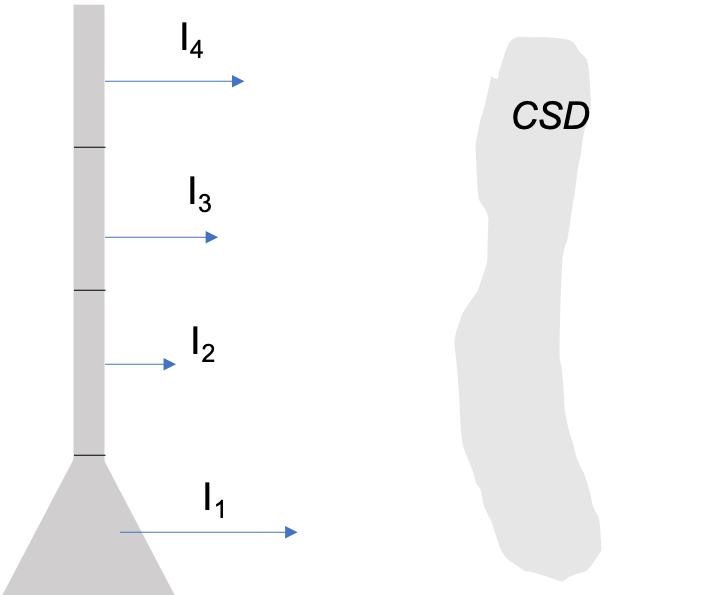
\includegraphics[width=0.3\textwidth]{Figures/VC/CSD.png}
\end{center}
\caption{\textbf{Neuronal current sources.}  {\bf (A)} When simulated on a numerical scheme, the transmembrane currents are known at a discrete set of neuronal segments, i.e., as a set of point sources.  {\bf (B)} As a mathematical generality, we can describe the transmembrane currents as a current source density (CSD) distribution, $C({\bf r},t)$. We note the sum of current entering/leaving a neuron is always zero, so that in {\bf (A)}, we must have that $I_1 + I_2 + I_3 + I_4 = 0$, and in {\bf (B)} we have that the spatial integral over $C$ must be zero.
}
\label{VC:fig:CSD}
\end{figure}
Volume conductor theory is essentially based on current continuity in the extracellular medium, i.e., the requirement that no net current can enter/leave a given point in space. Mathematically, current continuity implies that:
\begin{equation}
\nabla \cdot {\bf i_t}({\bf r}, t) = - C({\bf r}, t),
\label{VC:eq:CSD1}
\end{equation}
which is the same as we postulated previously in eq. \ref{Basics:eq:continuity1}. Here, ${\bf i_t}$ is the extracellular current density through the brain tissue, and $C$ is the current source density. What Eq. \ref{VC:eq:CSD1} essentially tells us, is that if a neuron outputs a current into a (infinitesimal) volume of space (the $C$ term), an equally large current leaves that volume as an extracellular current (the $\nabla \cdot {\bf i_t}$ term).

In this chapter, we shall assume that the extracellular current density is described by Ohm's law (eq. \ref{VC:eq:ohmici}). If we combine Eq. \ref{VC:eq:ohmici} and Eq. \ref{VC:eq:CSD1}, we get:

\begin{equation}
\nabla \left( \sigma_t({\bf r}, t) \nabla \phi({\bf r}, t) \right) = - C({\bf r}, t),
\label{VC:eq:CSD2}
\end{equation}

which simplifies to the more commonly used relation:
\begin{equation}
\sigma \nabla^2\phi({\bf r}, t) = - C({\bf r}, t),
\label{VC:eq:CSD3}
\end{equation}
in the less general case where the conductivity $\sigma_t$ is constant. Hence, if we know the distribution of neuronal current sources, we can integrate eq. \ref{VC:eq:CSD2} or eq. \ref{VC:eq:CSD3} to predict the electrical potential in the extracellular space surrounding the sources. 

As indicated above, the variables ${\bf i_t}$, $\sigma_t$ and $\phi$ can in general be functions of both position and time. However, for the remainder of this chapter, we shall for simplicity assume that $\sigma_t$ is constant. Furthermore, it is implicit in eq. \ref{VC:eq:CSD2} that the relationship between current sources and extracellular potentials is instantaneous (i.e., we can solve eq.  \ref{VC:eq:CSD2} at each time point independently), and in the remainder of the chapter we therefore only use the positional argument for ${\bf i_t}$ and $\phi$. 

In the following subsections, we show how VC-theory is used to compute $\phi$ in some idealized cases with a homogeneous extracellular medium, and then discuss how this theory can be expanded to more complex cases accounting for inhomogeneities. 


%%%%%%%%%%%%%%%%%%%%%%%%%%%%%%%%
\section{\blue{Infinite isotropic homogeneous extracellular medium}}
\label{sec:VC:isohomo}
\index{Conductivity!Homogeneous and isotropic}
%%%%%%%%%%%%%%%%%%%%%%%%%%%%%%%%

We shall now derive an expression for the extracellular potential $\phi$ in the case where the extracellular medium is infinite, isotropic and homogeneous. By homogeneous we mean that the conductivity $\sigma_t$ is the same everywhere in space, and by isotropic we mean that $\sigma_t$ is the same in all spatial directions. Although the extracellular medium in reality is neither infinite, nor strictly isotropic and homogeneous, this approximation may still in many cases give fairly good predictions of $\phi$.


%%%%%%%%%%%%%%%%%%%%%%%%%%%%%%%%
\subsection{\blue{Point source approximation}}
\label{sec:VC:pointsource}
\index{Point source approximation}

%%%%%%%%%%%%%%%%%%%%%%%%%%%%%%%%
We start by deriving the contribution to $\phi$ from a single neuronal point source $I_k$ at the point ${\bf r_k}=0$ (Fig. \ref{VC:fig:pointsource}A). 

\begin{figure}[!ht]
\begin{center}
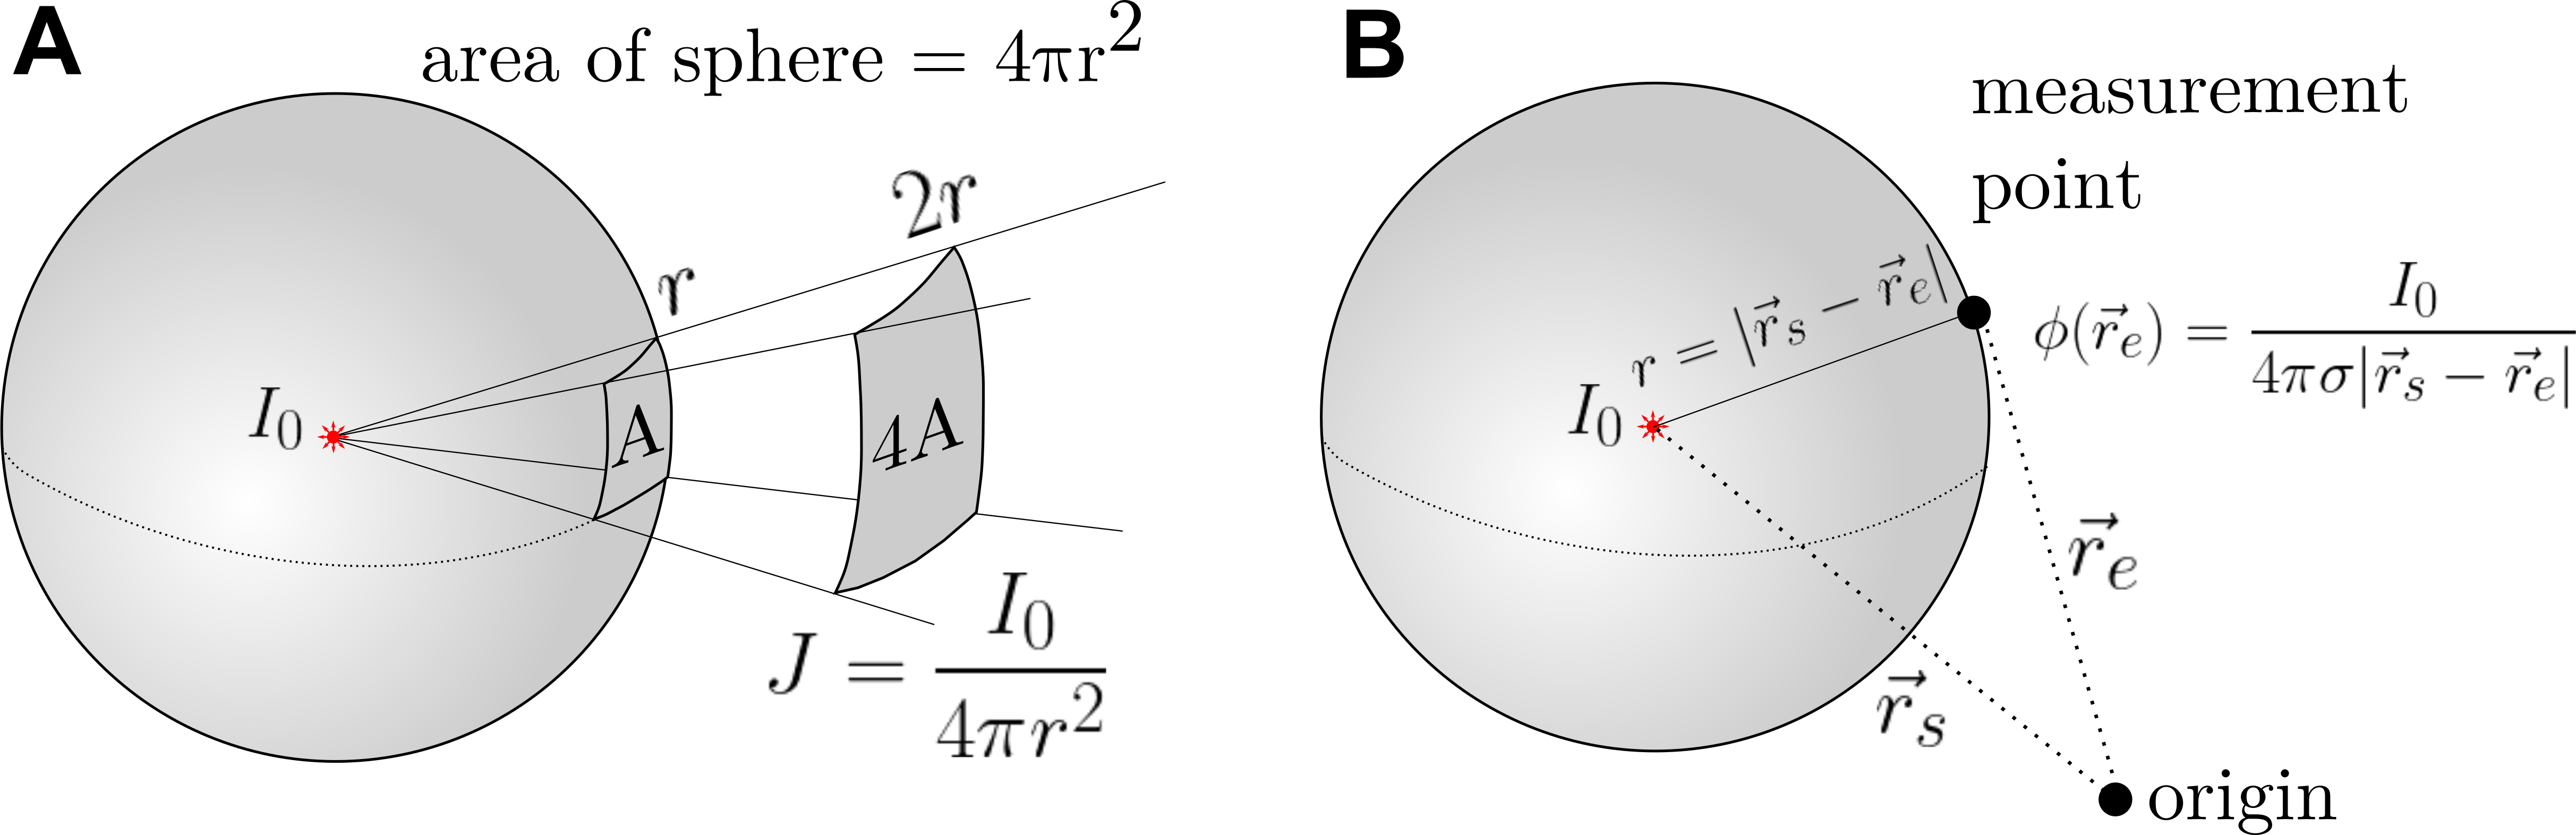
\includegraphics[width=0.8\textwidth]{Figures/VC/EP_from_pointsource_illustration.png}
\end{center}
\caption{\textbf{Extracellular potential from single neuronal point source current.} 
\tvnnote{Har laget utkast til figur. Noe slikt? } \ghnote{Praktfull, men trenger index $t$ paa $\sigma_t$, og $i_t$ erstatter J.}
}
\label{VC:fig:pointsource}
\end{figure}

Here, we could compute $\phi$ by solving eq. \ref{VC:eq:CSD3}. However, due to the spherical symmetry of this simple case, we can take a shorter path by realizing that the current density (eq. \ref{VC:eq:ohmici}) must radially directed, and that its magnitude must be solely a function of distance $r$ from the source:

\begin{equation}
i_t({\bf r}) = i_t(r) = -\sigma_t \frac{d\phi(r)}{dr}.
\end{equation}

Knowing this, we may find $\phi$ by simply demanding that net current $I_k$ injected into the center of the spherical volume with radius $r$ must equal the net current leaving through the surface of the volume, which in turn must equal the current density $i_t(r)$ at the surface multiplied with the surface area $4\pi r^2$. We then get the relationship:

\begin{equation}
I_k = -4\pi \sigma_t r^2  \frac{d\phi(r)}{dr} \, \iff \, \frac{d\phi(r)}{dr} = -\frac{I_k}{4\pi \sigma_t r^2 }.
\label{VC:eq:knut}
\end{equation}

To obtain the final solution for $\phi$, we integrate eq. \ref{VC:eq:knut} from $r$ to $\infty$:

\begin{equation}
\int_r^{\infty} \frac{d\phi(r')}{dr'} dr' = \int_r^{\infty} -\frac{I_k}{4\pi \sigma_t r'^2 } dr'.
\label{VC:eq:knut2}
\end{equation}
Since $\phi({\infty}) = 0$, this leads to the final expression:

\begin{equation}
\phi({\bf r}) = \phi(r) = \frac{I_k}{4\pi \sigma_t r},
\label{VC:eq:pointsource}
\end{equation}
where $r$ is the distance from the source.

In the above, we made things simple by assuming that the current source was placed in the origin ${\bf r} = 0$. For a point source located in an arbitrary point ${\bf r_k} $, the corresponding expression for the extracellular potential is:

\begin{equation}
\phi({\bf r}) = \frac{I_k}{4\pi \sigma_t |{\bf r-r_k}|},
\label{VC:eq:pointsource2}
\end{equation}

If we have several point-current sources, $I_{1}, I_2, I_3, ... $ in locations ${\bf r_1}, {\bf r_2}, {\bf r_3} ... $), their contributions add up linearly, and the potential in a point ${\bf r}$ is given by:

\begin{equation}
\phi({\bf r}) = \frac{I_1}{4\pi  \sigma_t {\bf |r-r_1|}} + \frac{I_2}{4\pi  \sigma_t {\bf |r-r_2|} } + \frac{I_3}{4\pi  \sigma_t {\bf |r-r_3|} } + ... = \sum_k \frac{I_k}{4\pi  \sigma_t {\bf |r-r_k|} }.
\label{VC:eq:pointsources}
\end{equation}


%%%%%%%%%%%%%%%%%%%%%%%%%%%%%%%%
\subsection{\blue{Line source approximation}}
\label{sec:VC:linesource}
\index{Line source approximation}

%%%%%%%%%%%%%%%%%%%%%%%%%%%%%%%%
Eq.~\ref{VC:eq:pointsources} is referred to as the point-source approximation \cite**{Holt1999,Pettersen2008a}, since it approximates the neuron as a set of point current sources, i.e., the neuron delivers to the extracellular space a singular current source per neuronal segment, located in the segment midpoint. 

A more sophisticated choice may be to assume that the transmembrane current is evenly distributed over the segment axis, a choice which is referred to as the line-source approximation \cite**{Holt1999,Linden2014}. The contribution to the extracellular potential from a current $I_k$ in a segment $k$ can be found analytically by integrating eq. \ref{VC:eq:pointsource} over the center-line axis of the compartment (see Appendix C in \cite**{Holt1998}). We here skip the derivation, but give the final solution. For a segment with length $\Delta s_k$, the contribution to the extracellular potential will be:

\begin{equation}
\phi({\bf r},t)_k = \frac{I_k}{4\pi \sigma_t} \int \frac{dr_k}{|{\bf r-r_k}|} = 
\frac{I_k}{4\pi \sigma_t \Delta s_k} \log \left| \frac{\sqrt{h_k^2+\rho_k^2}-h_k}{\sqrt{\ell_k^2+\rho_k^2}-\ell_k} \right|,
\label{VC:eq:linesource}
\end{equation}

Here $\rho_k$ is the distance perpendicular to the line segment, $h_k$ is the longitudinal distance from the end of the segment, and $\ell_k = \delta s_k + h_k$ is the longitudinal distance from the start of the segment (Fig.~\ref{VC:fig:line_source_illustration}). Eq. \ref{VC:eq:linesource} and Eq. \ref{VC:eq:pointsource} are the equivalent expressions where the transmembrane currents in a single neuronal segment are treated as a line source and point source, respectively. As for the point-source approximation, the contributions from several line-sources add up linearly. That is, if we have multiple segments $k$, the extracellular potential can be computed as:
\begin{figure}[!ht]
\begin{center}
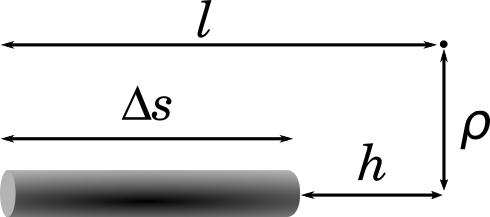
\includegraphics[width=0.4\textwidth]{Figures/VC/line_source_illustration.png}
\end{center}
\caption[]{\textbf{Line-source approximation.} 
\cite**{Holt1998} \tvnnote{Add subscripts?}
}
\label{VC:fig:line_source_illustration}
\end{figure}

\begin{equation}
\phi({\bf r},{\bf t}) = \sum_k \frac{I_k}{4\pi \sigma_t \Delta s_k} \log \left| \frac{\sqrt{h_k^2+\rho_k^2}-h_k}{\sqrt{\ell_k^2+\rho_k^2}-\ell_k} \right|,
\label{VC:eq:linesources}
\end{equation}

The line-source approximation can be expected to give a better prediction of $\phi$ than the point-source approximation at points in space that are very near neuronal membranes, especially when it comes to predicting rapid fluctuations in $\phi$, such as the extracellular action potential signature \cite**{Holt1999}. At points further away from membranes, the two approaches give converging predictions, see Fig.~\ref{VC:fig:point_vs_linesource}.

\begin{figure}[!ht]
\begin{center}
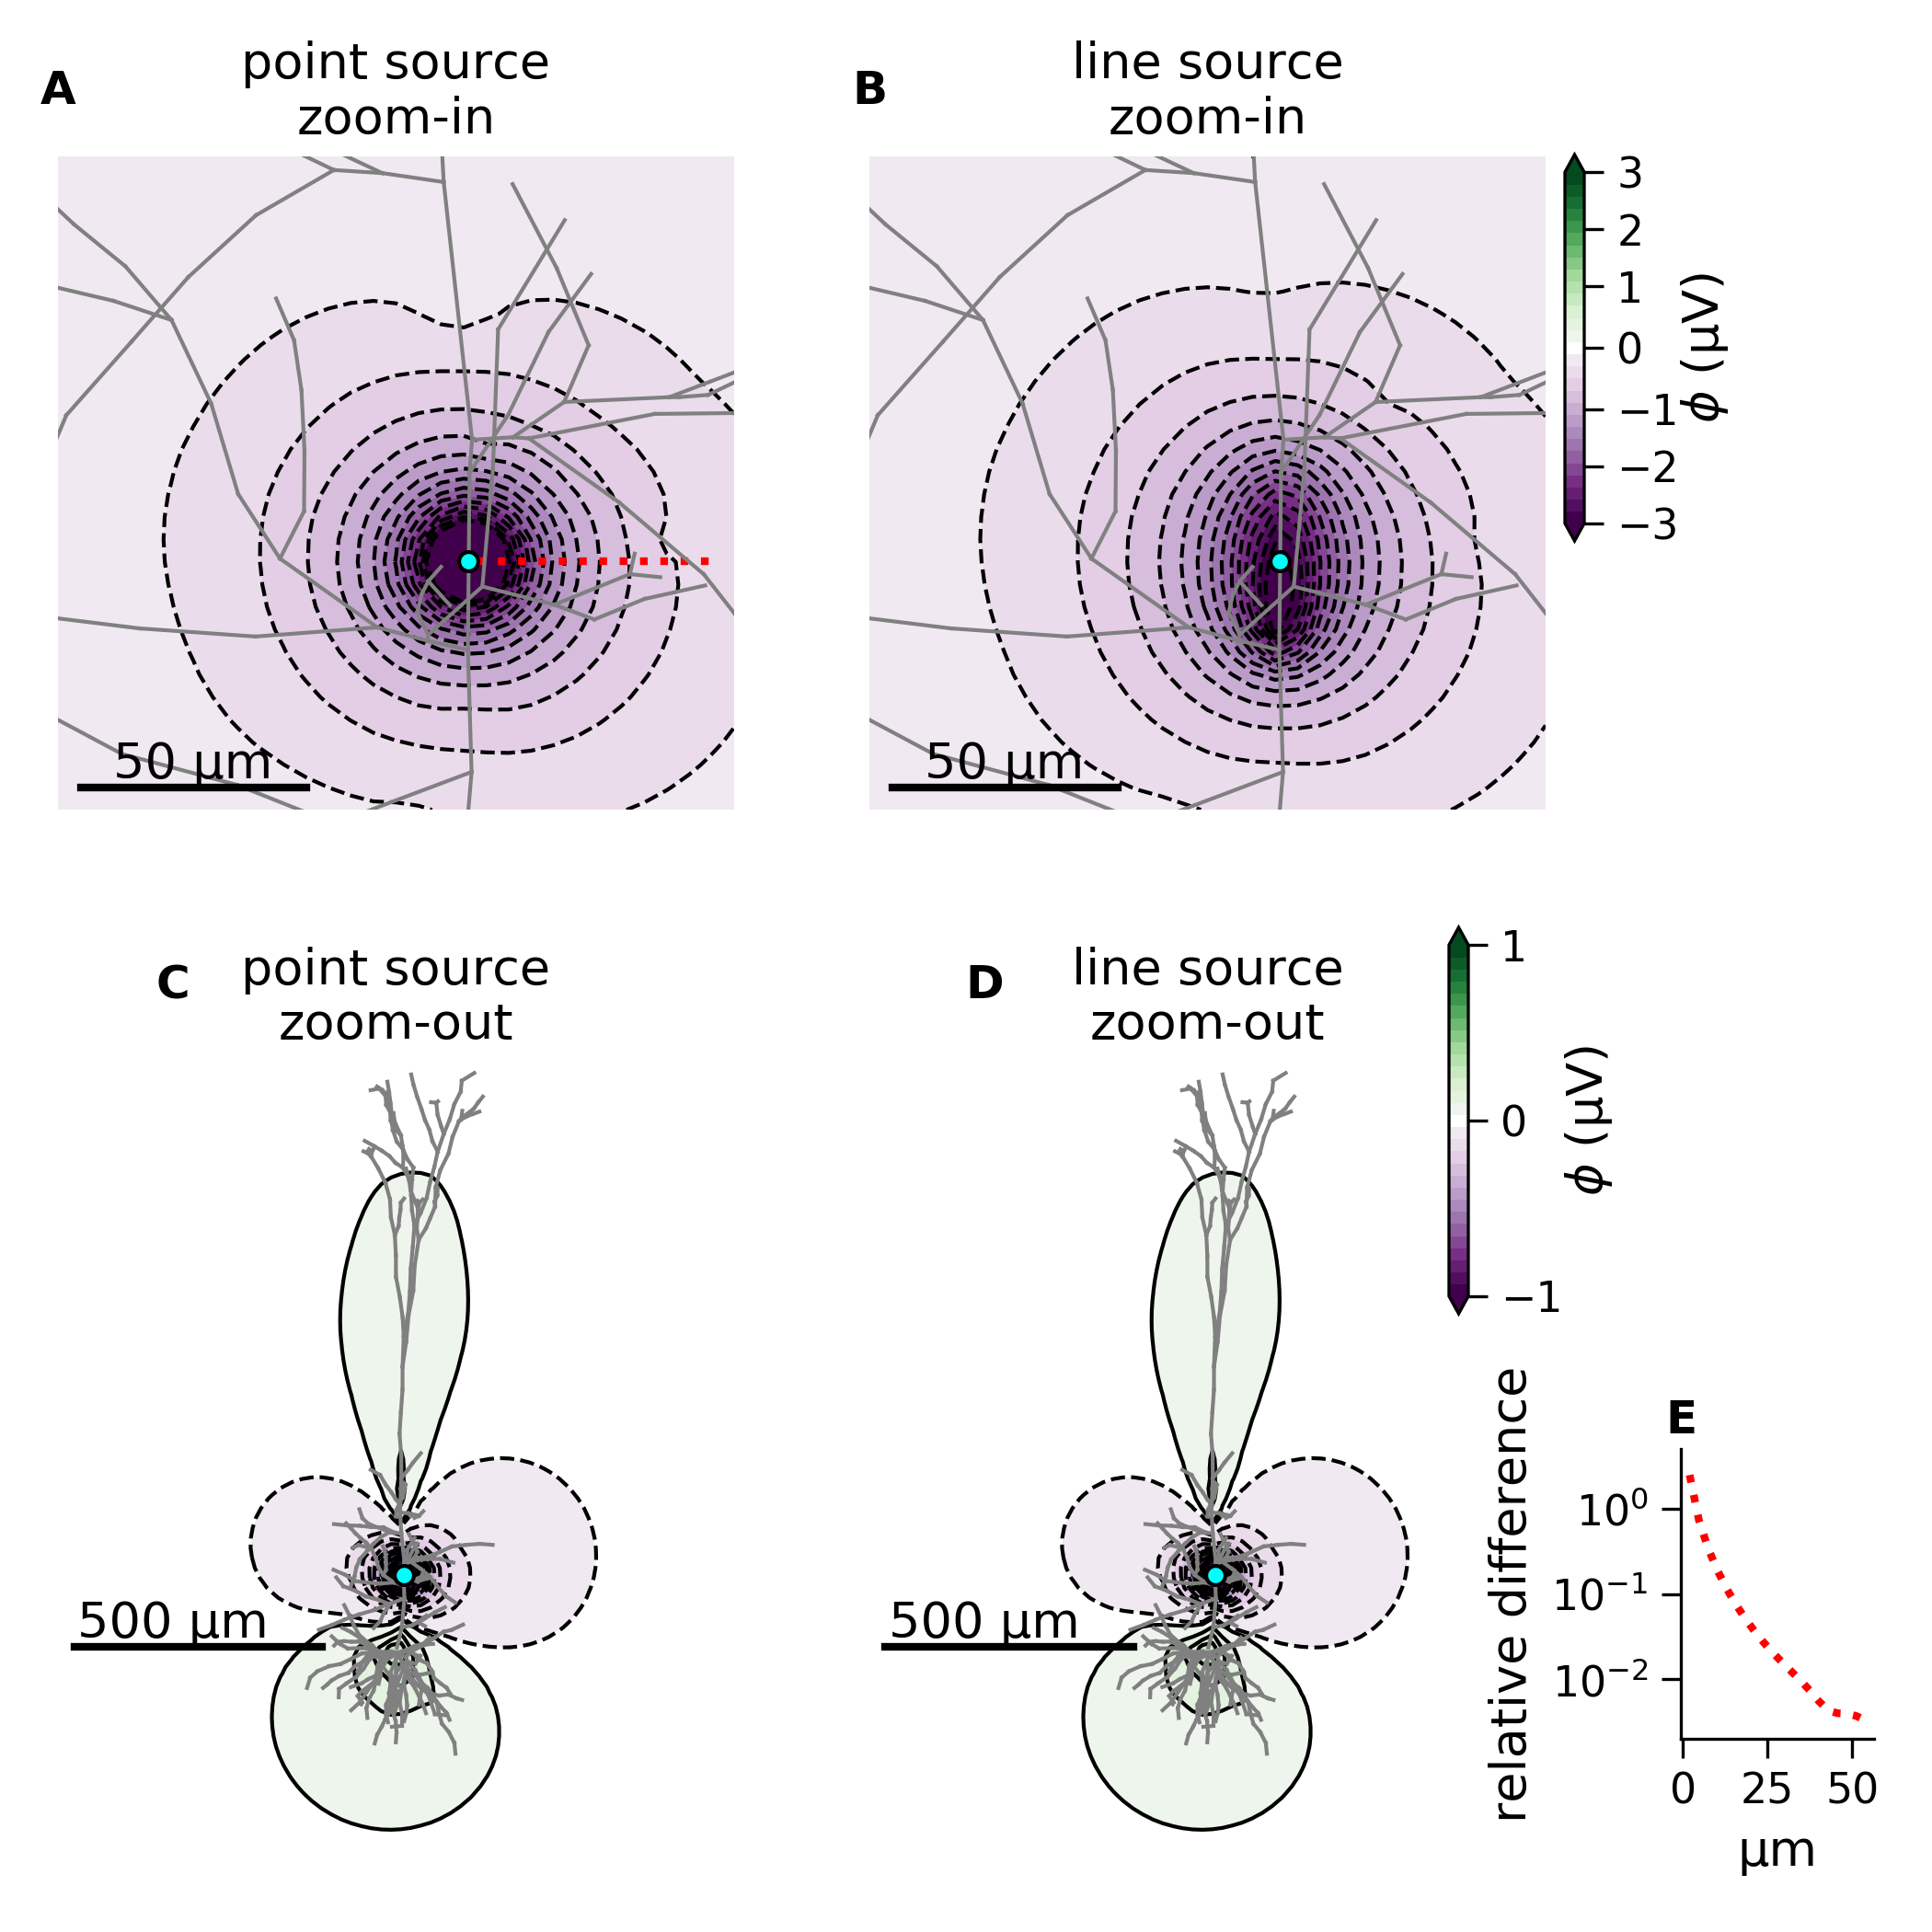
\includegraphics[width=0.7\textwidth]{Figures/VC/fig_point_versus_linesource.png}
\end{center}
\caption[]{\textbf{Point- versus line-source approximation.}
}
\label{VC:fig:point_vs_linesource}
\end{figure}

%%%%%%%%%%%%%%%%%%%%%%%%%%%%%%%%
\subsection{\blue{Current-source-density description}}
\label{sec:VC:CSD}
\index{Current source density}
%%%%%%%%%%%%%%%%%%%%%%%%%%%%%%%%
The forward modelling formulas in Eq. \ref{VC:eq:pointsources} and \ref{VC:eq:linesources} can be expressed more generally in terms of the CSD. The starting point is then eq. \ref{VC:eq:CSD3}, which for a homogeneous and isotopic medium can be written: 

\begin{equation}
\nabla^2 \phi({\bf r}) = - \frac{C({\bf r})}{\sigma_t}
\label{VC:eq:CSD4}
\end{equation}

Since this is a linear differential equation, we may solve it by first finding its Green's function, i.e., the solution to an impulse response $C({\bf r}) = I' \delta^3({\bf r-r'})$, where $\delta^3({\bf r})$ is the Dirac delta function in three dimensions, and $I'$ is the current source at this location. The general solution can then be expressed as a convolution over such Green's functions. Thus, we first seek the solution to: 

\begin{equation}
\nabla^2 \phi({\bf r}) = - \frac{I' \delta^3({\bf r-r'})}{\sigma_t}.
\label{VC:eq:CSD5}
\end{equation}

We already listed the solution to this in eq. \ref{VC:eq:pointsource2}, but we here provide a more rigorous derivation. We start by by integrating both sides of eq. \ref{VC:eq:CSD5} over an arbitrary 3D volume containing the source:

\begin{equation}
\iiint_V \nabla^2\phi({\bf r}) \,dV =  - \frac{I'}{\sigma_t} \iiint_V \ \delta^3({\bf r-r'}) \, dV,
\label{VC:eq:marit}
\end{equation}

By the definition of the delta-function, the right hand side of equation \ref{VC:eq:marit} is simply $I'/\sigma$. Using Gauss' theorem, we can convert the volume integral on the left hand side of eq. \ref{VC:eq:marit} to a surface integral, so that eq. \ref{VC:eq:marit} becomes:

\begin{equation}
\oiint_{S} \nabla\phi({\bf r}) \cdot \, d{\bf S}  = - \frac{I'}{\sigma_t},
\label{VC:eq:berit1}
\end{equation}

To solve this, it is convenient to chose the volume that we integrate over to be a sphere centered at the source location ${\bf r'}$, and with radius $R = |{\bf r-r'}|$ (Fig. \ref{VC:fig:pointsource}B). Due to the symmetry of problem, we then know that the electrical potential is the same for all ${\bf r}$ on the surface of the sphere, so that $\phi({\bf r}) = \phi(R)$. We also know that its gradient $\nabla\phi({\bf r}) = d\phi(R)/dR$ is constant over the surface, and perpendicular to the surface increment $d{\bf S}$. If we use this, eq. \ref{VC:eq:berit1} becomes:
\begin{equation}
\oiint_{S} \frac{d\phi(R)}{dR} d{S}  = - \frac{I'}{\sigma_t},
\label{VC:eq:berit1ogenhalv}
\end{equation}
which has the solution:
\begin{equation}
4\pi R^2 \frac{d\phi(R)}{dR} = \frac{I'}{\sigma_t}
\label{VC:eq:berit2}
\end{equation}
If we integrate this from $R$ to $\infty$, and use that $\phi(\infty) = 0$, we get:
\begin{equation}
\phi(R) = \phi({\bf r}) = \frac{I'}{4\pi \sigma_t R}.
\label{VC:eq:berit3}
\end{equation}
We may now insert back for $\phi(R)= \phi({\bf r})$ and $R = |{\bf r-r'}|$ to obtain the desired Green's function:

\begin{equation}
\phi({\bf r})= \frac{I'}{4\pi \sigma_t |{\bf r-r'}|},
\label{VC:eq:berit4}
\end{equation}
As earlier stated, the solution for a general CSD can be expressed as a convolution over the Green's function, so that:

\begin{equation}
\phi({\bf r}) = \frac{1}{4\pi \sigma_t}\iiint_V \frac{C({\bf r'})}{|{\bf r}-{\bf r'}|} \,dV, 
\label{VC:eq:csds}
\end{equation}
where the volume integral runs over all sources. Here, $C$ represents whatever approximation one used for the current sources, and eq. \ref{VC:eq:csds} is the continuous counterpart to eq. \ref{VC:eq:pointsources}. If we describe the CSD as a sum of point sources, i.e.,  $C({\bf r}) = \sum_k I_k \delta^3({\bf r} - {\bf r_k})$, eq. \ref{VC:eq:csds} reduces to eq.\ref{VC:eq:pointsources}.


%%%%%%%%%%%%%%%%%%%%%%%%%%%%%%%%
\section{\orange{SN: Dipole approximation}}
\label{sec:VC:dipole}
\ghnote{GH: Jeg skrev en skisse til dette kapittelet, men fint om SN kan gaa gjennom.}
%%%%%%%%%%%%%%%%%%%%%%%%%%%%%%%%
The \textit{dipole approximation} \index{Dipole approximation} is an alternative to eq. \ref{VC:eq:pointsources} for predicting the extracellular potential. The approximation is good provided that the "measuring point" for $\phi$ is far away from the source-sink distribution that it originates from, like in the case of EEG.

To be more precise, if the distance from the center of the volume containing the current sources to the measurement point is larger than the maximal distance from volume center to any source [cite - find Jackson!], we can reformulate eq. \ref{VC:eq:pointsources} by using the the multipole expansion \cite**{Nunez2006}:

\begin{equation}
\phi(R) = \frac{C_{monopole}}{R} + \frac{C_{dipole}}{R^2} + \frac{C_{quadrupole}}{R^3} + \frac{C_{octupole}}{R^4} + ...
\label{VC:eq:multipole}
\end{equation}
where $R$ is the distance from the center of the source distribution, $C_{monopole}$ is the monopolar contribution of the CSD to $\phi$, $C_{dipole}$ is the dipolar contribution from the CSD to $\phi$, and so on. The derivation of this expression can be found in Appendix \ref{app:dipoleappendix}. 

As we explained in Section \ref{sec:Neuron:membranecurrents}, the net sum of currents over a neuronal membrane is always zero, meaning that the monopolar contribution, i.e., first term in eq. \ref{VC:eq:multipole}, vanishes. Furthermore, the quadrupole, octopole and higher-order contributions to $\phi$ decay rapidly with distance $R$. Provided that we are sufficiently far away from the source distribution, $\phi$ can therefore be well approximated by dipole contribution alone:

\begin{equation}\label{VC:eq:CDA}
\Phi(\mathbf{R}) \approx \frac{1}{4 \pi \sigma_t} \frac{|\mathbf{p}| \cos \theta}{R^2},
\end{equation}
where we have expressed $C_{dipole}$ in terms of the current dipole moment ($\mathbf{p}$), the angle ($\theta$) between the current dipole moment and the distance vector ($\mathbf{R}$), as explained in Appendix \ref{app:dipoleappendix}. 

The current dipole moment is a function of the sum of all the transmembrane currents in a neuron \cite**{Pettersen2008,Pettersen2014,Nunez2006}: 
\begin{equation}\label{VC:eq:dipole}
\mathbf{p} = \sum_{k=1}^N I_k \mathbf{r}_k.
\end{equation}
For example, if we have a simple two-compartmental (and purely dipolar) neuron with a current sink $-I$ at location $\mathbf{r}_1$ and a current source $I$ at location $\mathbf{r}_2$, the current dipole moment can be formulated as $\mathbf{p} = -I\mathbf{r}_1 + I\mathbf{r}_2 = I(\mathbf{r}_2 - \mathbf{r}_1) = I\mathbf{d}$. Here $\mathbf{d}$ is the distance vector between the current sink and the current source, giving the length $d$ and direction of the current dipole. 

As we mentioned above, the current dipole approximation is only applicable when we are at some distance away from the source distribution. As a rule of thumb, the approximation is though to be good when $R$ is three to four times greater than the dipole length: $R > 3d$ or $R > 4d$ \cite**{Nunez2006}. It has been found to work well for predicting the extracranial EEG signal, but less well for intracranial electrocorticography (ECoG) \cite**{naess2020biophysical}.


\section{\orange{TVN: Modelling recording electrodes}}
\label{sec:VC:electrodes}
\index{Electrode model}
We have demonstrated how we can use volume conductor theory to make predictions about the extracellular potentials at any point in space following some neural activity. However, in experiments these extracellular potentials must be measured through some kind of measurement electrode. The presence of such a measurement electrode might itself affect the measured potentials in several different ways, depending on both the electrode and the extracellular potential that is being measured. Here we present a short review of different approaches to model such effects.

\tvnnote{Litt usikker på om jeg bruker alle begreper riktig i dette avsnittet} Recording electrodes essentially consist of an electrode surface in direct contact with neural tissue, connected with a wire to an amplifier that measures the potential relative to ground or a reference electrode \cite**{Martinsen2008}, see Fig.~\ref{VC:fig:elec_circuit}. For recording electrodes to accurately measure the potential at the electrode surface, the measurement electrodes themselves must have a very high conductivity so that no potential drop occurs from the measurement site to the amplifier. The electrodes are therefore typically made of a highly conductive metal like silver or platinum, and the potential directly on the inside the electrode surface is in practice homogeneous. The amplifier must however have a near zero conductivity, so that a negligible amount of current will cross the tissue-electrode interface, as this can cause electrode polarization effects\index{Electrode polarization} \cite**{Schwan1992,Moulin2008,Ishai2013,Martinsen2008}. 
The homogeneous potential inside the recording electrode ideally corresponds to a spatial average of the potential across the outer surface of the electrode \cite**{Ness2015,Vermaas2020b}\tvnnote{Bør finne lærebok-referanse til dette?}. 

\begin{figure}[!ht]
\begin{center}
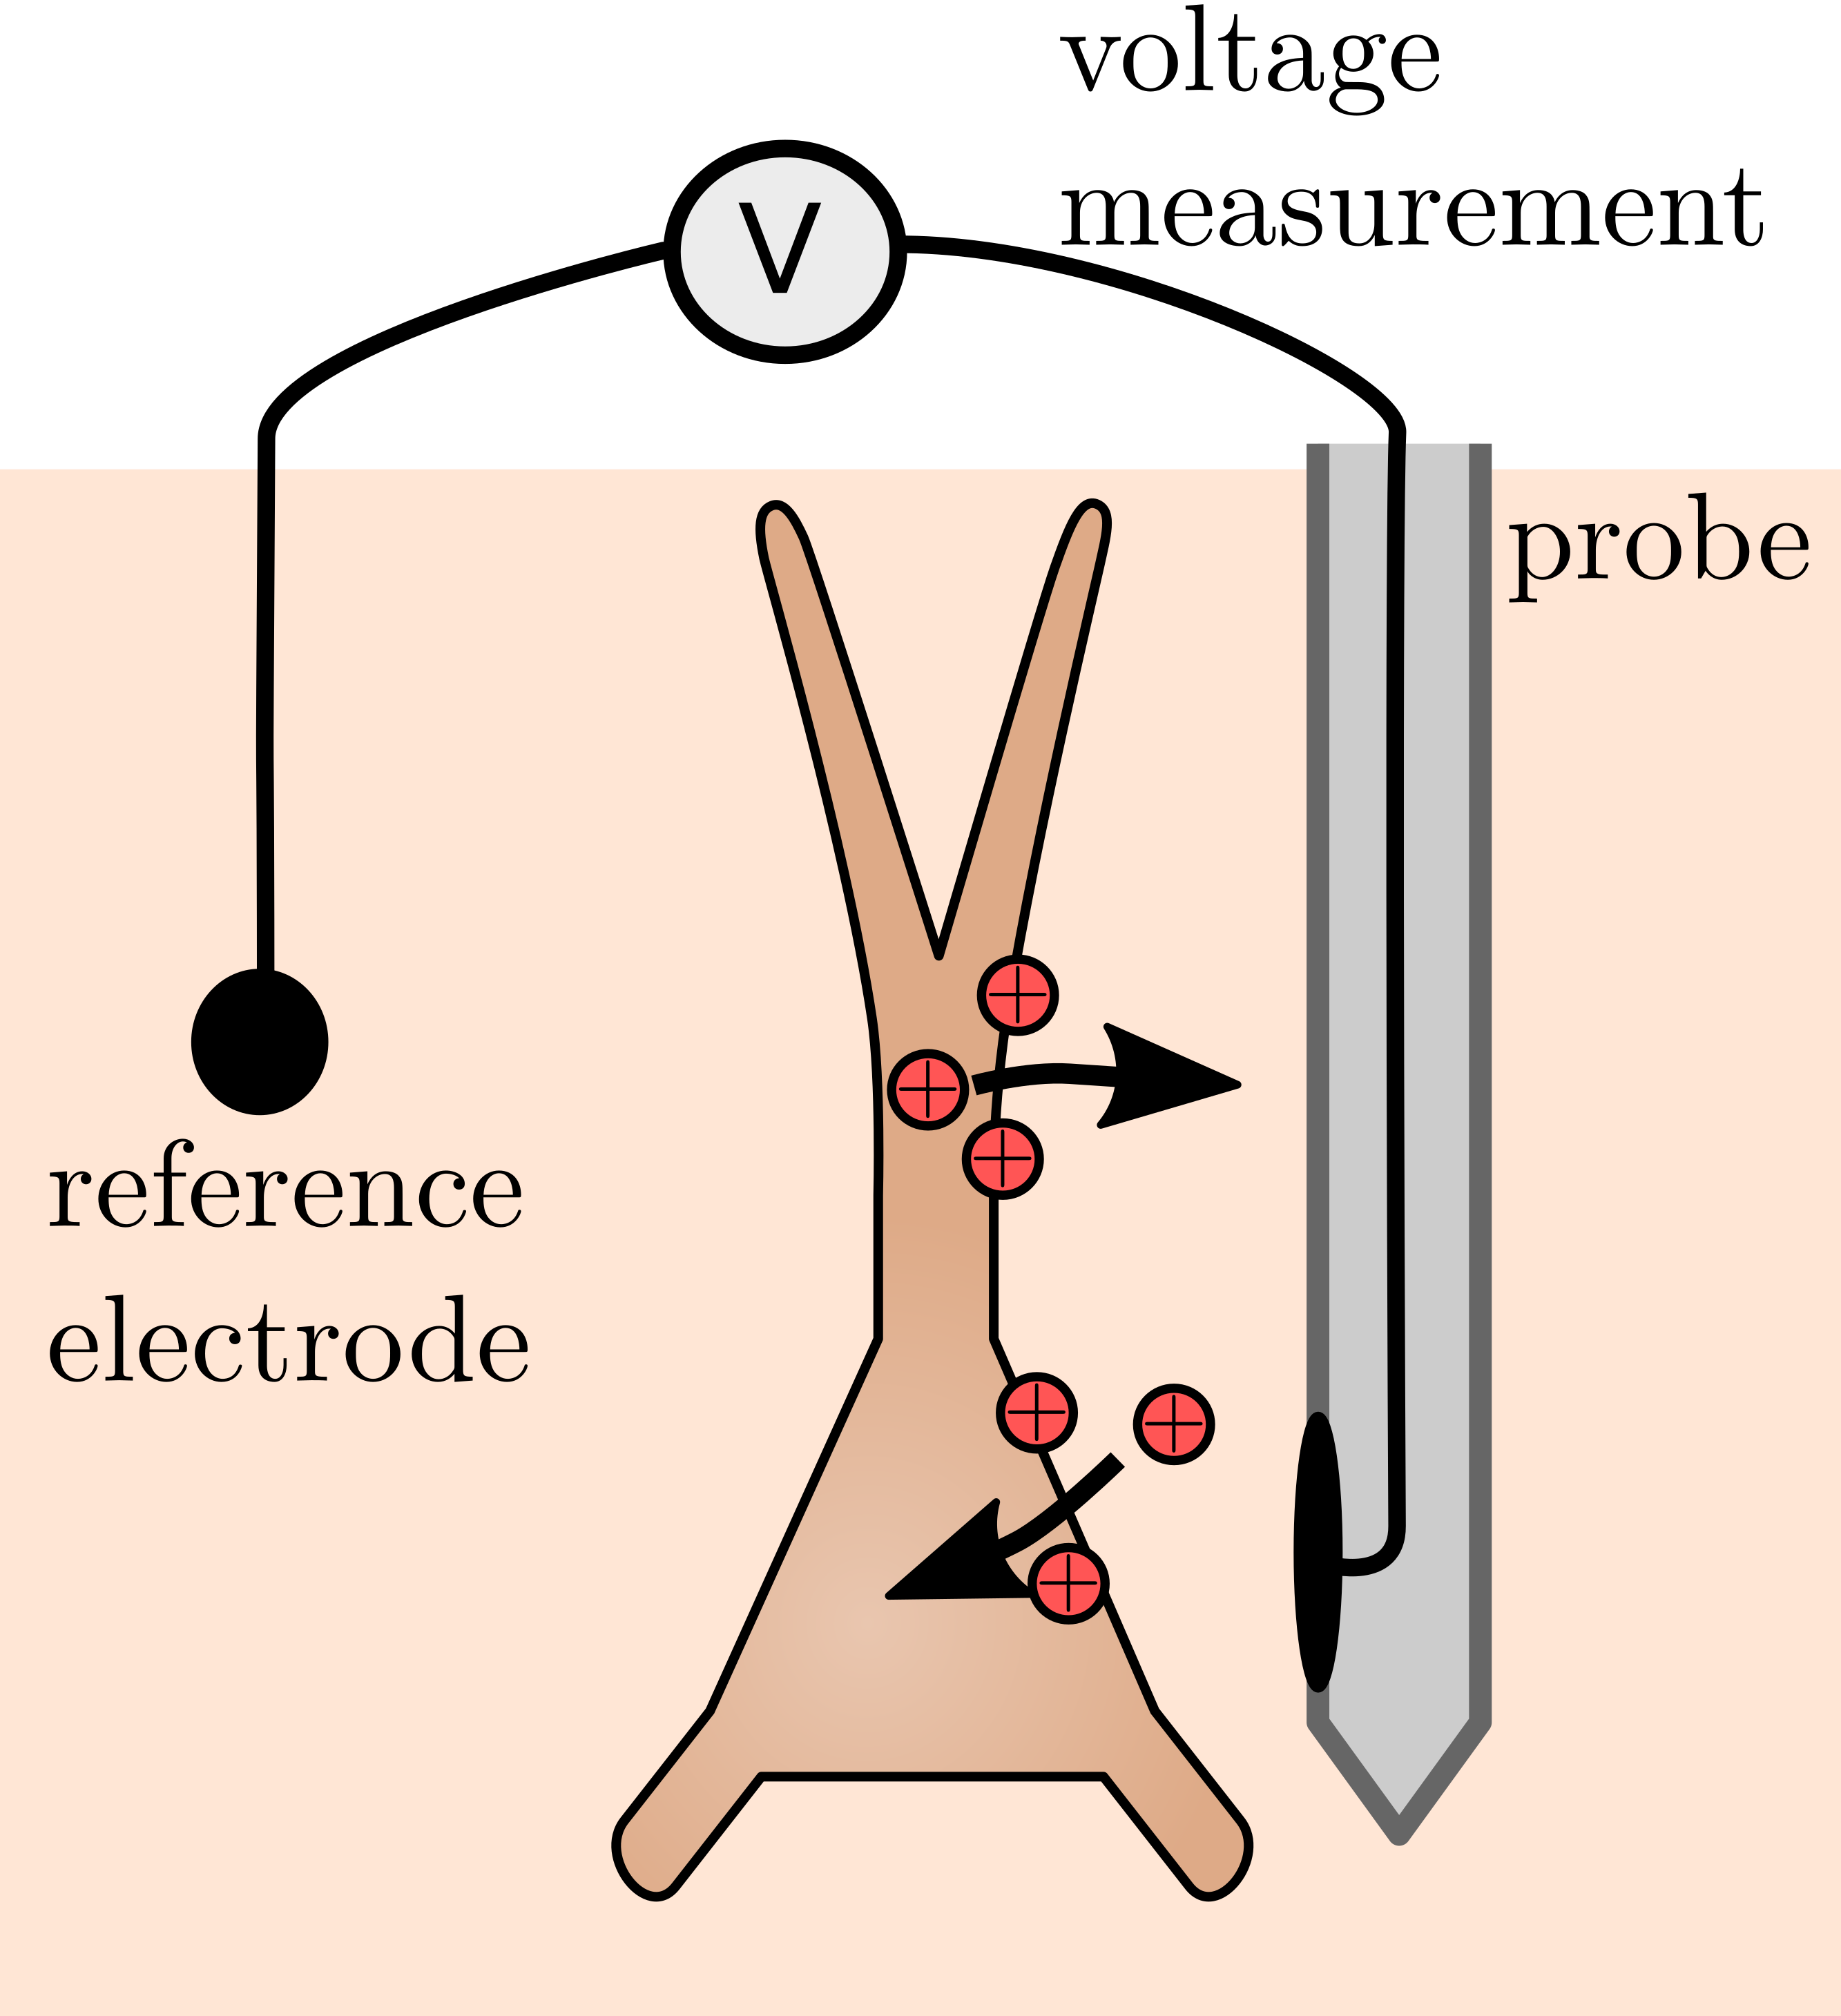
\includegraphics[width=0.4\textwidth]{Figures/VC/rec_elec_circuit.png}
\end{center}
\caption[]{\textbf{Illustration of recording circuit}
Electric potential is measured between recording electrode and reference electrode, and represents the energy required to move a positive test charge from the reference electrode and to the measurement electrode. If, say, positive ions are leaving the extracellular medium (and entering a cell) in the vicinity of the recording electrode, then the energy needed to move a positive charge to the measurement electrode is negative, that is, one can gain energy by moving the charge there.  
}
\label{VC:fig:elec_circuit}
\end{figure}

A possible concern is whether the electrode impedance or other electrode properties can distort measured extracellular potentials, through introducing unintentional temporal filtering effects on the recorded potentials. Effectively, this would amount to the potential on the inside of the electrode surface being different from the (spatial average of the) potential on the outside of the electrode, and therefore not represent the "true" extracellular potential.
For example, note that recording electrodes are typically unable to measure static (DC) potentials, or capture changes slower than $\sim$ 0.1 Hz. Such DC potentials can be present in neural tissue, and can often arise in simulated extracellular potentials from cell models with active conductances, for example because of the $I_{\rm h}$-current \cite**{Ness2016}. In such cases, the simulated baseline (or mean) extracellular potential is typically subtracted from the extracellular potentials to effectively remove the unobservable DC-potential.

Apart from this, it has been convincingly argued that, provided that the proper recording equipment is used, electrode impedance or other electrode properties should not substantially distort recorded potentials \cite**{Martinsen2008,Moulin2008,Nelson2008,Nelson2010}. 
  Note that this only applies to recording electrodes, and that substantially more complex electrode models might be needed to accurately represent current stimulation electrodes because of electrode polarization \cite**{McIntyre2001,Martinsen2008,Joucla2012}.
In essence, the complication stems from that in electronics the electric charge is carried by electrons, while in neural tissue the electric charge is carried by positive and negative ions. For low frequencies, which do not favor capacitive currents, this change of charge carrier can be problematic, resulting in electrode polarization. 
  Modelling electrode polarization effects will often require numerically comprehensive approaches, like the Finite Element Method (FEM) \index{Finite Element Method}\cite**{Buitenweg2003,Moulin2008,Joucla2014,Vermaas2020a}, and/or careful calibration to experimental recordings \cite**{Gabriel1996,Martinsen2008,Miceli2017},
and this topic is not covered here.

Under the assumption that the proper recording equipment is used \cite**{Nelson2008,Nelson2010}, electrode properties can still affect the recorded potential. For example, if the extracellular potential changes across the outer surface of the recording electrode, this can introduce a spatial filtering effect on the measured potentials. In practice, this means for example that extracellular action potentials (which are very spatially confined) will be less prominent on electrodes with diameters larger than $\sim$30~$\mu$m \cite**{Moffitt2005,Moulin2008}, see Fig.~\ref{VC:fig:electrode_size}.

\begin{figure}[!ht]
\begin{center}
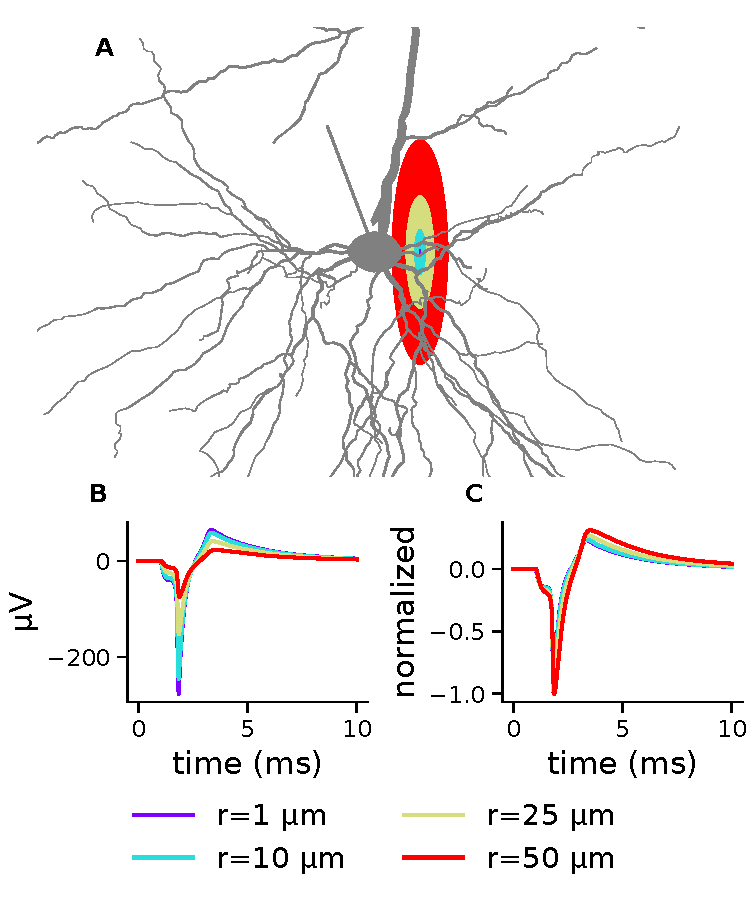
\includegraphics[width=0.6\textwidth]{Figures/VC/fig_elec_size_effect.pdf}
\end{center}
\caption[]{\textbf{Effect of electrode size.}
Bigger recording electrodes can cause smaller and broader EAPs.
}
\label{VC:fig:electrode_size}
\end{figure}

\subsection{\orange{Point-electrode approximation}}
\index{Point-electrode}
The most straightforward and also most common approach when modeling extracellular recordings is to use the ideal point electrode approximation. This corresponds to  
ignoring any potential effect from recording electrodes or electrode shanks, and calculating the extracellular potential  at single points. For relatively small micro-electrodes inserted into neural tissue, this has been found to be a reasonable approximation \cite**{Ness2015,Buccino2019b}\tvnnote{Legg til sitering fra ikke-oss}.

\ghnote{Tror vi maa forklare at punktet vaart er et punkt i en coarse-grained beskrivelse av tissue. "Punktet" i vaar utregning tilsvarer en midling over et mikrometerstort omraade rundt punktet s.a. utslaget ikke er avhengiv av hvorvidt det er 1, 2, 3 eller 40 nm til naermeste membran. Den samme midlingen gjoeres av smaa elektroder. Saa "point" betyr i denne sammenhengen at vi allokerer elektrodemaalingen til punktet i sentrum av elektroden, og at elektrodens tilstedevaerelse ikke paavirker hva midlingen over dette omraadet vil vaere?}

\subsection{\orange{Disc-electrode approximation}}
\index{Disc-electrode approximation}
In some cases recording electrodes are large enough that the extracellular potential varies substantially across the electrode surface. In such cases, we can use the point-electrode approximation to calculate the potential at many points across the electrode surface and compute the average potential. This is typically referred to as the disc-electrode approximation \cite**{Linden2014,Ness2015}. 

By taking into account the physical extent of the electrodes, the disc-electrode approximation can account for spatial filtering effects. However, very close to electrodes the electrodes can themselves affect the close-by extracellular potential, since they represent a region of a highly conductive material in contact with the tissue being measured from. 
The effect of the presence of highly conductive electrodes can be investigated using FEM, and \citeasnoun**{Ness2015} found that the disc-electrode approximation was fairly accurate for estimating measured potentials from a point current source more than $\sim$2 times the electrode radius away from the electrode.

In certain cases, like in ECoG \index{ECoG} measurements from the cortical surface, the recording electrodes are both large ($\sim$~2-5~mm diameter) and close to the neuronal sources (the thickness of the human cortex is $\sim$3~mm). In such cases the electrode properties can therefore be expected to have large effect on measured potentials, see for example  \cite**{Vermaas2020b,Rogers2020}.

\subsection{\orange{Effect of the electrode probes}}

Large multi-contact electrode probes can be expected to have a substantial effect on close-by extracellular potentials, since it represents a large non-conducting volume \cite**{Mechler2012,Buccino2019b}. It has been demonstrated that such large probes can amplify or dampen recorded potentials from nearby cells by almost a factor of two, depending on whether the cell was in front of or behind the electrode shank \cite**{Moffitt2005,Buccino2019b}.

%%%%%%
\section{\blue{Approximations used in VC theory}}
\label{sec:VC:approximations}
%%%%%%%%%%%%%%%%%%%%%%%%%%%%%%%%
The VC theory presented in this chapter relies on several assumptions and approximations. Firstly, the theory is based on the quasi-static approximation of Maxwell's equations (see Section \ref{sec:VC:quasistatic} for more on this). Secondly, the the extracellular medium is assumed to be linear, so that the current density is proportional to the electrical field (see Section \ref{sec:VC:LinEx} for more on this). Thirdly, extracellular currents are assumed to be exclusively due to Ohmic drift, although other currents could in principle be present (see Section \ref{sec:VC:onlyohmic} for more on this). Fourthly, when applying VC theory, one typically assumes that there is no (ephaptic) feedback from extracellular potentials on the neural activity (see Section \ref{sec:VC:ephaptic} for more on this). Finally, the extracellular conductivity was throughout this chapter assumed to be isotropic, homogeneous and frequency independent, but it is possible to relax these assumptions. Given its important role, we have devoted an entire chapter of this book to the extracellular conductivity (Chapter \ref{sec:Sigma}), where we discuss how the VC theory can be applied also to cases with an anisotropic medium and non-homogeneous medium.

\subsection{\blue{Quasi-static approximation of Maxwell's equations}}
\label{sec:VC:quasistatic}
\index{Quasi-static approximation to Maxwell's equations}
In the quasi-static approximation to Maxwell's equations, one neglects terms with the time derivatives of the electric (${\bf E}$) and magnetic (${\bf B}$) fields. For linear materials with instantaneous response properties, Maxwell's (macroscopic) equations for the curl of the electric and magnetic fields can then be simplified to:
\begin{equation}
\nabla \times {\bf E} = - \frac{\partial {\bf B}}{\partial t}  \approx 0, 
\label{VC:eq:maxE}
\end{equation}
and
\begin{equation}
\nabla \times {\bf B} = \mu{\bf i} + \mu \epsilon \frac{\partial {\bf E}}{\partial t} \approx  \mu {\bf i} ,
\label{VC:eq:maxB}
\end{equation}
where $\mu$ and $\epsilon$ are the permeability and permittivity of the medium respectively. It follows from eq. \ref{VC:eq:maxE} that the static electric field is conservative, and related to an extracellular potential through,
\begin{equation}
{\bf E} = \nabla \cdot \phi.
\label{VC:eq:conservative}
\end{equation}
The quasi-static approximation appears to be well-justified for the relatively low frequencies relevant for brain signals, below about 10 kHz \cite**{Nunez2006,Grodzinsky2011}.


\subsection{\blue{Linear extracellular medium} }
\label{sec:VC:LinEx}
\index{Extracellular medium! Linear}

In a linear extracellular medium, the relationship between the current density and the electric field is given by:
\begin{equation}
{\bf i} = \sigma {\bf E}.
\label{VC:eq:bertil}
\end{equation}
This relation is constitutive, meaning that it is observed in nature rather than derived from any physical principle \cite**{Nunez2006,Pettersen2012}. It is quite general, and $\sigma$ can here in principle be anisotropic (i.e., a tensor, accounting for different conductivities in different directions), inhomogeneous (position dependent), and complex (accounting for capacitive effects). We note that eq. \ref{VC:eq:bertil} is generally only valid in the frequency domain, while in the time domain, ${\bf i}$ must be given as a temporal convolution of $\sigma$ and ${\bf E}$ \cite**{Bedard2009}. However, if $\sigma$ is frequency independent (this assumption is discussed further below), eq. \ref{VC:eq:bertil} will also be valid in the time domain.

Eq. \ref{VC:eq:bertil} is essentially Ohm's law for a volume conductor. If we combine it with the quasi-static approximation (i.e., with eq. \ref{VC:eq:conservative}), we get a current density given by ${\bf i} = \sigma \nabla \phi$, which is what we assumed for extracellular tissue currents in the beginning of this chapter (eq. \ref{VC:eq:ohmici}).


\subsection{\blue{Extracellular currents are exclusively due to Ohmic drift}}
\label{sec:VC:onlyohmic}
When basing the VC theory on eq. \ref{VC:eq:ohmici}, we assumed that extracellular currents are mediated exclusively by Ohmic drift. In principle, a current density could have additional contributions from diffusion of ions, advection currents and displacement currents:

\begin{equation}
{\bf i} = {\bf i^{ohm}} + {\bf i^{dif}} + {\bf i^{adv}} + {\bf i^{dis}}, 
\label{VC:eq:generalcurrent}
\end{equation}

The advective current, 
\begin{equation}
{\bf i^{adv}} = F \rho {\bf u}, 
\label{VC:eq:iadv}
\end{equation}
is the current that arises in a bulk solution if the solution has a charge density $\rho$ that it drags along with it due to a bulk flow with velocity ${\bf u}$, while the displacement current,
\begin{equation}
{\bf i^{dis}} = \frac{\partial \rho}{\partial t},
\label{VC:eq:idis}
\end{equation}
represents the capacitive effect of a medium that allows local charge accumulation, so that $\rho$ can vary with time.  

For the physiological conditions of the extracellular solution, the charge relaxation time, i.e., the time it takes for $d\rho/dt$ to decay to zero when responding to a change in the electric field, is in the order of 1 ns \cite**{Grodzinsky2011,Gratiy2017}. This means that the displacement current (eq. \ref{VC:eq:idis}) will mainly be important under conditions when the electrical field varies with frequencies in the GHz range. As the relevant fields with physiological origin vary with frequencies that are orders of magnitude lower than this, the displacement current can safely be neglected. Related to this, the actual charge accumulation that takes place during a relaxation time of 1 ns is very small. For most practical purposes it is a therefore good approximation to assume that the extracellular medium is electroneutral \cite**{Solbra2018}, which means that $\rho = 0$ so that the advective current becomes zero. Hence, for practical purposes, it is safe to assume that both the displacement current (eq. \ref{VC:eq:idis}) and the advective current (eq. \ref{VC:eq:iadv}) give negligible contributions to extracellular dynamics. A more physically rigorous argument for this was given in \citeasnoun**{Gratiy2017}. 

The diffusive current \index{Diffusive current},
\begin{equation}
{\bf i^{dif}} = -F \sum_k z_k D_k \nabla c_k,
\label{VC:eq:idif}
\end{equation}
represents the current that arrises when ions (with valence $z_k$ and diffusion constants $D_k$) diffuse along extracellular concentration gradients ($\nabla c_k$), and carry along with them a net charge. Diffusive currents are neglected in standard VC theory under the assumption that they are much smaller than Ohmic drift currents at the coarse grained scale of brain tissue. By estimates, the effect of diffusion on $\phi$ is most likely small under normal conditions, so that one might generally make quite good predictions with a VC theory that neglects them \cite**{Halnes2016,Gratiy2017}. 

However, diffusive currents can have a notable impact on $\phi$ in physiological conditions with large concentration gradients \cite**{Halnes2016,Gratiy2017}. Diffusive effects on $\phi$ may therefore be particularly relevant under pathological conditions such as epilepsy, stroke and spreading depression, which are associated with dramatic shifts in local extracellular concentrations (see e.g.,  \cite**{Somjen2001,Frohlich2008,Wei2014,Ayata2015}). 

To account for diffusive effects, one needs to compute not only the electrical potential, but also the ion concentration dynamics of all involved ions at all points in space. This can not be done using VC theory in the standard form presented here, but can be done using Finite Element Methods \cite**{Solbra2018}. We go through the theory for modelling electrodiffusive systems in Chapter \ref{sec:Eldiff}.


\subsection{\orange{No ephaptic effects} }
\label{sec:VC:ephaptic}
\index{Ephaptic effects}
The standard workflow when modeling the extracellular potential ($\phi$) involves two steps: In Step 1 one uses the multicompartment (MC) formalism (cf. Chapter \ref{sec:Neuron}) to compute the transmembrane currents in all neuronal compartments. In Step 2, one uses VC theory (eq. \ref{VC:eq:pointsources}) to estimate the resulting $\phi$. Since the fundamental equation in the MC formalism (eq. \ref{Neuron:eq:multimain}) was derived under the assumption that $\phi=0$, this two-step approach is evidently inconsistent. 

In reality, the activity of a neuron will affect the membrane potential of both neighboring neurons and itself through the extracellular potential that it creates. Such effects of the extracellular potential on the neurodynamics are called \textit{ephaptic}. As we discussed in Section \ref{sec:Neuron:HHCassumptions}, $\phi$ is typically much smaller than the membrane potential, and ephaptic effects are therefore commonly assumed to be negligibly small. Provided that this is true, the two-step approach works well. 

Importantly, the negligence of ephaptic effects when using the two-step scheme is implicit in the way that the neurons are modeled (Step 1), and not in the physical fundament of the VC theory (Step 2). The VC theory does not in itself make any assumption regarding ephaptic effects being present or not. Hence, the the extracellular potential should satisfy eq. \ref{VC:eq:pointsources} or \ref{VC:eq:csds} regardless of whether or not ephaptic effects were accounted for when the neural current sources were computed. As our main focus is on the extracellular potential, we will therefore stick with the two-step scheme throughout most of this book.